\documentclass{article}
\usepackage[utf8]{inputenc}
\usepackage[T1]{fontenc}
\usepackage{geometry}
\usepackage{hyperref}
\usepackage{graphicx}
\graphicspath{ {pictures/} }
\hypersetup{
    colorlinks,
    citecolor=black,
    filecolor=black,
    linkcolor=black,
    urlcolor=black
}
\geometry{a4paper}
\usepackage[english]{babel}
\title{Quantum Computing}
\author{Marta Bubel Ewelina Kolba}
\date{21-05-2022}
\begin{document}
\maketitle
Implementation a simple version of various logic functions and the Deutsch two qubit quantum algorithm.
\newpage
%spis tresci--------------------------------------------------------
\renewcommand{\contentsname}{Table of contents}
\tableofcontents
\newpage
\section{Introduction to Quantum Computing}
Quantum Computers are different from the digital computing that drives today's data centers, cloud environments, PCs and other devices. Digital computation requires data to be encoded into binary digits (bits), each of which is always in one of two definite states (0 or 1). However, quantum computation uses quantum bits (qubits), which can be in multiple states simultaneously. As a result, operations on qubits can amount to a large number of calculations in parallel. It has been shown that in theory, some specific problems should be solable in much less time on a quantum computer than using the best known algorithms for a conventional computer. Here are four key concepts that are the foundation of quantum computing.
\subsection{Superposition}
Classical physics can be either o or 1 bit. In quantum physics a qubit would be bot 0 and 1 and spin simultaneously up and down.
\subsection{Entanglement}
Entanglements gives quantum computing the ability to scale exponentially. If one qubit simultaneosly represents two states, two qubits represents four states when coupled together. They can no longer be treated independently, they now form a coupled or entangled, super state. As more qubits link together, the number of states exponentially increase, which could lead to a computer with astronomically large computing power.
\subsection{Fragility}
Quantum states are quite fragile. If you measure, observe, touch ot peturb any of these states, they collapse to a classical state. The states don't stick around for very long, which is why quantum computers are currently hard to build.
\subsection{No cloning}
A corrollary to fragility is the "No cloning theorem". In classical physics, if we have two bits, one can copy or eavesdrop and recreate the information. In contrast, the information entangled within a set of qubits will be lost if someone tries to observe or copy them. A quantum state cannot be copied without the sender or receiver realizing this. This concept serves as the basis of quantum communications.
\newpage
\section{Logic gates}
A logic gate is an idealized or physical device implementing a Boolean function, a logical operation performed on one or more binary inputs that produces a single binary output. 
Logic circuits include such devices as multiplexers, registers, arithmetic logic units (ALUs), and computer memory, all the way up through complete microprocessors, which may contain more than 100 million gates.
\subsection{Classical logic gates}
%--------------------------------------
\subsubsection{NOT}
\begin{figure}[h]
\begin{center}
\begin{minipage}[b]{4cm}
\centering
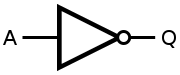
\includegraphics[width=2cm]{not_gate.png}\\\textit{NOT - gate}
\end{minipage}
\begin{minipage}[b]{2cm}
\centering
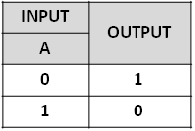
\includegraphics[width=2cm]{not_truthtable.png}\\\textit{NOT - Truth Table}
\end{minipage}
\end{center}
\end{figure}
%----------------------------------------
\subsubsection{AND}
\begin{figure}[h]
\begin{center}
\begin{minipage}[b]{4cm}
\centering
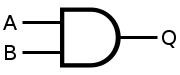
\includegraphics[width=2cm]{and_gate.png}\\\textit{AND - gate}
\end{minipage}
\begin{minipage}[b]{2cm}
\centering
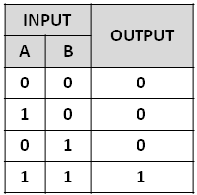
\includegraphics[width=2cm]{and_truthtable.png}\\\textit{AND - Truth Table}
\end{minipage}
\end{center}
\end{figure}
%--------------------------------------------
\subsubsection{OR}
\begin{figure}[h]
\begin{center}
\begin{minipage}[b]{4cm}
\centering
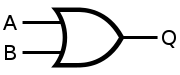
\includegraphics[width=2cm]{or_gate.png}\\\textit{OR - gate}
\end{minipage}
\begin{minipage}[b]{2cm}
\centering
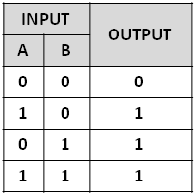
\includegraphics[width=2cm]{or_truthtable.png}\\\textit{OR - Truth Table}
\end{minipage}
\end{center}
\end{figure}
%--------------------------------------------
\newpage
\subsubsection{NAND}
\begin{figure}[h]
\begin{center}
\begin{minipage}[b]{4cm}
\centering
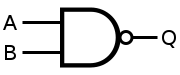
\includegraphics[width=2cm]{nand_gate.png}\\\textit{NAND - gate}
\end{minipage}
\begin{minipage}[b]{2cm}
\centering
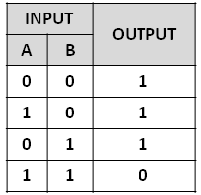
\includegraphics[width=2cm]{nand_truthtable.png}\\\textit{NAND - Truth Table}
\end{minipage}
\end{center}
\end{figure}
%--------------------------------------------
\subsubsection{NOR}
\begin{figure}[h]
\begin{center}
\begin{minipage}[b]{4cm}
\centering
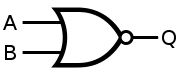
\includegraphics[width=2cm]{nor_gate.png}\\\textit{NOR - gate}
\end{minipage}
\begin{minipage}[b]{2cm}
\centering
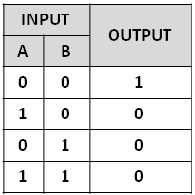
\includegraphics[width=2cm]{nor_truthtable.png}\\\textit{NOR - Truth Table}
\end{minipage}
\end{center}
\end{figure}
%--------------------------------------------
\subsubsection{XNOR}
\begin{figure}[h]
\begin{center}
\begin{minipage}[b]{4cm}
\centering
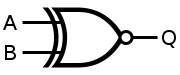
\includegraphics[width=2cm]{xnor_gate.png}\\\textit{XNOR - gate}
\end{minipage}
\begin{minipage}[b]{2cm}
\centering
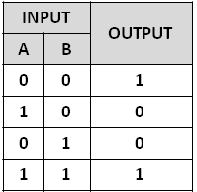
\includegraphics[width=2cm]{xnor_truthtable.png}\\\textit{XNOR - Truth Table}
\end{minipage}
\end{center}
\end{figure}
\newpage
%--------------------------------------------
\section{Deutsch algorithm}
\newpage
%bibligrafia
%\section*{Bibliography}
\begin{thebibliography}{x}
  % \bibitem{<biblabel>} <citation>
  \bibitem{citeA}
    {\scshape Author, A}, {\itshape A title}, Journal of So-and-So, 2000.
  \bibitem{citeB}
    {\scshape Someone, B}, {\itshape Another title}, Book of books, 1900.
\addcontentsline{toc}{section}{References}
\end{thebibliography}
\end{document}